\documentclass[11pt]{article}

\usepackage{amsmath,amssymb,mathtools}
\usepackage[margin=1in]{geometry}
\usepackage{enumitem}
\usepackage{xcolor}
\usepackage{microtype}
\usepackage{graphicx}
\usepackage{tikz,float}
\usepackage{subcaption}
\usepackage{amsthm}
\usepackage{hyperref}
\usepackage{array}
\usepackage{pgfplots}

\usetikzlibrary{shapes.geometric, arrows.meta, positioning, calc, decorations.markings}
\tikzset{
	block/.style={rectangle, draw, text width=6em, text centered, rounded corners, minimum height=10mm},
	sum/.style={circle, draw, node distance=1.5cm},
	line/.style={draw, -{Stealth[length=2.5mm, width=1.5mm]}}
}

\usepgfplotslibrary{groupplots}
\pgfplotsset{compat=1.18}

\pgfplotsset{
	myaxes/.style={
		axis lines=middle,
		axis line style={-latex},
		grid=major,
		grid style={gray!15},
		minor grid style={gray!35},
		xlabel style={at={(ticklabel* cs:1)}, anchor=north west},
		ylabel style={at={(ticklabel* cs:1)}, anchor=south east},
		every axis plot/.append style={thick}
	},
	myplotstyle/.style={
		width=14cm,
		height=7cm,
		axis lines=middle,
		axis line style={-Stealth},
		grid=both,
		minor tick num=1,
		major grid style={draw=gray!30},
		minor grid style={draw=gray!15},
		tick label style={font=\small, fill=white, inner sep=1.5pt},
		xlabel={$t$},
		ylabel={$x(t)$},
		xlabel style={anchor=north east, font=\small},
		ylabel style={anchor=south east, font=\small},
		samples=401,
	}
}

\newtheoremstyle{mynote}
{6pt}      % Space above
{6pt}      % Space below
{}          % Body font (normal, not italic)
{}          % Indent amount
{\bfseries} % Theorem head font
{.}         % Punctuation after theorem head
{.5em}      % Space after theorem head
{}          % Theorem head spec
\theoremstyle{mynote}
\newtheorem{definition}{Definition}
\newtheorem{proposition}{Proposition}
\newtheorem{example}{Example}
\newtheorem{remark}{Remark}
\newtheorem{theorem}{Theorem}
\newtheorem{corollary}{Corollary}

\newcommand{\T}{\mathcal{T}}
\newcommand{\R}{\mathbb{R}}
\newcommand{\Z}{\mathbb{Z}}
\newcommand{\C}{\mathbb{C}}
\newcommand{\conv}{\ast}
\newcommand{\dt}{\,\dd t}
\newcommand{\dd}{\mathrm{d}}
\newcommand{\imp}{\delta}
\newcommand{\sinc}[1]{\frac{\sin(\pi #1)}{\pi #1}}


\DeclareMathOperator{\rect}{rect}
\DeclareMathOperator{\Ev}{Ev}
\DeclareMathOperator{\Od}{Od}
\DeclareMathOperator{\sgn}{sgn}
\DeclareMathOperator{\step}{u}
\DeclareMathOperator{\tri}{tri}


\begin{document}
	% Reset figure counter for this lecture
	\renewcommand{\thefigure}{11.\arabic{figure}}
	
	% --- TITLE BLOCK ---
	\thispagestyle{empty}
	\noindent
	\begin{tabular*}{\textwidth}{l @{\extracolsep{\fill}} r}
		\textbf{Signals and Systems} & \textbf{Lecture 11} \\
		\textit{Dr. Ghandi Manasra and Ahmed Rabei} & \textit{Fall 2025} \\
	\end{tabular*}
	\hrule
	\vspace{0.4cm}
	\begin{center}
		\Large\textbf{Lecture 11: The Continuous-Time Fourier Transform (CTFT)}
	\end{center}
	\vspace{0.4cm}
	
	\section*{Reference}
	Oppenheim \& Willsky, \textit{Signals and Systems}, Chapter 4, Sections 4.0--4.1
	
	\section*{Review of Lecture 10}
	\begin{itemize}[noitemsep]
		\item LTI systems as frequency-domain multipliers
		\item Complex exponentials as eigenfunctions
		\item Filtering concept and filter types
	\end{itemize}
	
	\section*{11.1 Introduction}
	
	The Fourier Series provides a powerful tool for analyzing periodic signals, but many important signals are \textbf{aperiodic}. Today, we extend our frequency-domain analysis to include these signals through the \textbf{Continuous-Time Fourier Transform (CTFT)}.
	
	We can think of an aperiodic signal $x(t)$ as the limit of a periodic signal $\tilde{x}(t)$ as the period $T_0$ goes to infinity.

	Consider a periodic signal $\tilde{x}(t)$ with Fourier series representation:
	\[
	\tilde{x}(t) = \sum_{k=-\infty}^{\infty} a_k e^{jk\omega_0 t}
	\]
	where $\omega_0 = \frac{2\pi}{T_0}$ and the Fourier coefficients are:
	\[
	a_k = \frac{1}{T_0} \int_{-T_0/2}^{T_0/2} \tilde{x}(t)e^{-jk\omega_0 t} \dt
	\]
	
\subsection*{11.1.1 The Envelope Function:}
	
	Each $a_k$ tells us "how much" of frequency $k\omega_0$ is in our signal. As the period gets longer, these frequencies become more and more closely spaced.
	
	Let's define an \textbf{envelope function} $X(j\omega)$ by scaling the Fourier coefficients by $T_0$:
	\[
	X(jk\omega_0) = T_0 a_k = \int_{-T_0/2}^{T_0/2} \tilde{x}(t)e^{-jk\omega_0 t} \dt
	\]
	
	This envelope function is like a smooth curve that connects all our discrete frequencies. It represents the continuous frequency content of our signal.
	
	Rewriting the synthesis equation in terms of this envelope:
	\[
	\tilde{x}(t) = \sum_{k=-\infty}^{\infty} \frac{1}{T_0} X(jk\omega_0) e^{jk\omega_0 t} = \frac{1}{2\pi} \sum_{k=-\infty}^{\infty} X(jk\omega_0) e^{jk\omega_0 t} \omega_0
	\]
	
\subsection*{11.1.2 Taking the Limit:}
	
	As $T_0 \to \infty$:
	\begin{itemize}[noitemsep]
		\item $\tilde{x}(t) \to x(t)$, as the repetition is eliminated
		\item $\omega_0 = \frac{2\pi}{T_0} \to 0$  - the frequency spacing shrinks
		\item $k\omega_0$ becomes a continuous variable $\omega$ - discrete impulses become a smooth curve
		\item The sum becomes an integral
	\end{itemize}
	

	This leads to the \textbf{Fourier Transform pair}:
	
	\section*{11.2 The Continuous-Time Fourier Transform (CTFT)}
	
	\begin{definition}
		For a signal $x(t)$, the \textbf{analysis equation} (Fourier Transform) is:
		\[
		X(j\omega) = \int_{-\infty}^{\infty} x(t)e^{-j\omega t} \dt
		\]
		The \textbf{synthesis equation} (Inverse Fourier Transform) is:
		\[
		x(t) = \frac{1}{2\pi} \int_{-\infty}^{\infty} X(j\omega)e^{j\omega t} \dd\omega
		\]
	\end{definition}
	
	\textbf{Intuitive Interpretation:} The analysis equation can be understood as measuring the similarity or correlation between the signal $x(t)$ and the complex exponential $e^{j\omega t}$ for each frequency $\omega$. When $x(t)$ has strong components at frequency $\omega$, the integral produces a large value for $X(j\omega)$; when there are no such components, the integral is small or zero.
	
	\subsection*{11.2.1 Convergence Conditions}
	
	The Fourier transform exists if the \textbf{Dirichlet conditions} are satisfied:
	
	\begin{enumerate}[noitemsep]
		\item \textbf{Absolute integrability:} $\int_{-\infty}^{\infty} |x(t)| \dt < \infty$
		\item $x(t)$ has a finite number of maxima, minima, and discontinuities in any finite interval
	\end{enumerate}
	
	\begin{remark}
		These are \textbf{sufficient} but not \textbf{necessary} conditions. Many signals that violate these conditions still have Fourier transforms (e.g., periodic signals, impulses).
	\end{remark}
	
	\section*{11.3 Examples of the CTFT}
	
	\subsection*{11.3.1 Decaying Exponential}
	
	Let $x(t) = e^{-at}u(t)$ for $a > 0$.
	
	\begin{align}
		X(j\omega) &= \int_{0}^{\infty} e^{-at}e^{-j\omega t} \dt \\
		&= \int_{0}^{\infty} e^{-(a+j\omega)t} \dt \\
		&= \left[ -\frac{1}{a+j\omega}e^{-(a+j\omega)t} \right]_0^\infty \\
		&= \frac{1}{a+j\omega}
	\end{align}
	
	\subsection*{11.3.2 Rectangular Pulse}
	
	Let $x(t) = \begin{cases} 1, & |t| < T_1 \\ 0, & |t| > T_1 \end{cases}$.
	
	\begin{align}
		X(j\omega) &= \int_{-T_1}^{T_1} e^{-j\omega t} \dt \\
		&= \left[ -\frac{1}{j\omega}e^{-j\omega t} \right]_{-T_1}^{T_1} \\
		&= \frac{e^{j\omega T_1} - e^{-j\omega T_1}}{j\omega} \\
		&= \frac{2\sin(\omega T_1)}{\omega} = 2T_1 \sinc{\frac{\omega T_1}{\pi}}
	\end{align}
	
	\begin{figure}[H]
		\centering
		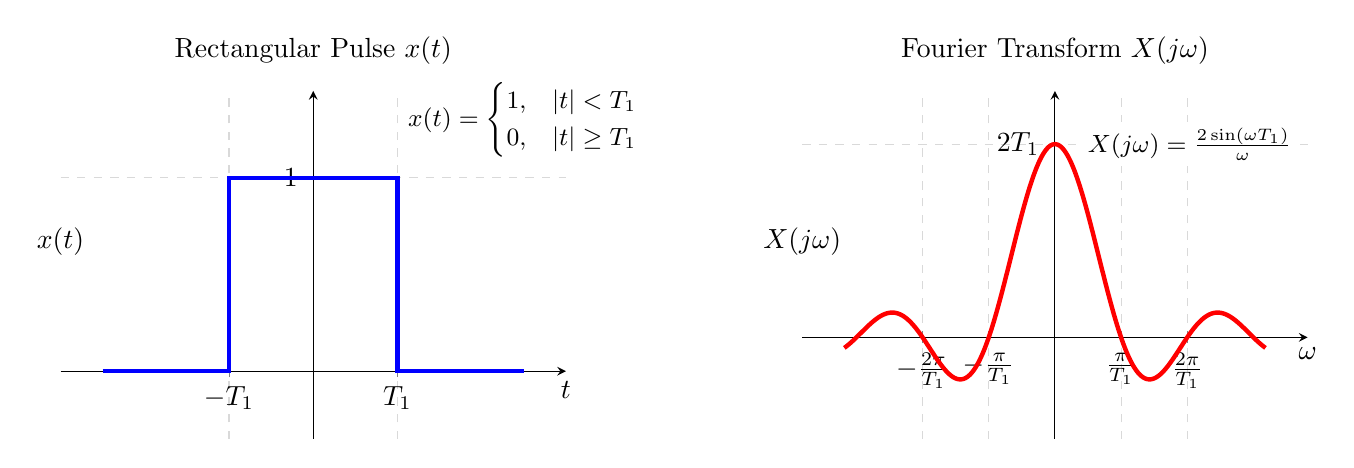
\begin{tikzpicture}
	% Define the pulse half-width T_1 for easy modification
	\def\T{2} 
	
	\begin{groupplot}[
		group style={
			group size=2 by 1,
			horizontal sep=3cm,
		},
		width=8cm,
		height=6cm,
		domain=-5:5,
		samples=500,
		axis lines=middle,
		enlargelimits=true,
		clip=false,
		xlabel style={at={(axis cs:6,0)},anchor=north},
		ylabel style={at={(axis description cs:0,.5)},anchor=south},
		grid=major,
		grid style={dashed, gray!30},
		]
		
		% Rectangular Pulse in Time Domain
		\nextgroupplot[
		title={Rectangular Pulse $x(t)$},
		xlabel={$t$},
		ylabel={$x(t)$},
		xtick={-\T, 0, \T},
		xticklabels={$-T_1$, $0$, $T_1$},
		ytick={0, 1},
		ymin=-0.2,
		ymax=1.3,
		]
		\addplot[blue, ultra thick] coordinates {(-5,0) (-\T,0) (-\T,1) (\T,1) (\T,0) (5,0)};
		\node[fill=white, inner sep=2pt, font=\small] at (axis cs:5,1.3) {\(x(t) = \begin{cases} 1, & |t| < T_1 \\ 0, & |t| \geq T_1 \end{cases}\)};
		
		% Sinc Function in Frequency Domain (Fourier Transform)
		\nextgroupplot[
		title={Fourier Transform $X(j\omega)$},
		xlabel={$\omega$},
		ylabel={$X(j\omega)$},
		xtick={-2*pi/\T, -pi/\T, 0, pi/\T, 2*pi/\T},
		xticklabels={$-\frac{2\pi}{T_1}$, $-\frac{\pi}{T_1}$, $0$, $\frac{\pi}{T_1}$, $\frac{2\pi}{T_1}$},
		ytick={0, 2*\T},
		yticklabels={$0$, $2T_1$},
		ymin=-1.5,
		ymax=4.5,
		]
		% Corrected sinc plot with zero handled explicitly
		\addplot[red, ultra thick] 
		{(x==0) ? 2*\T : 2*sin(deg(\T*x))/x};
		\node[fill=white, inner sep=2pt, font=\small] at (axis cs:3.2, 4) {\(X(j\omega) = \frac{2\sin(\omega T_1)}{\omega}\)};
		
	\end{groupplot}
\end{tikzpicture}
		\caption{Rectangular pulse and its Fourier transform (sinc function)}
		\label{fig:rectangular_pulse}
	\end{figure}
	
	\subsection*{11.3.3 Unit Impulse}
	
	Let $x(t) = \delta(t)$.
	
	Using the sifting property:
	\[
	X(j\omega) = \int_{-\infty}^{\infty} \delta(t)e^{-j\omega t} \dt = e^{-j\omega \cdot 0} = 1
	\]
	
	\newpage
	\subsection*{11.3.4 Constant Signal}
	
	Let $x(t) = 1$ for all $t$.
	
	This signal is not absolutely integrable, so its Fourier transform cannot be found by direct evaluation of the analysis integral. Instead, we can find the transform by working backward from the synthesis equation (the inverse Fourier transform).
	
	Let's propose that the transform of $x(t) = 1$ is a scaled Dirac delta function, $X(j\omega) = c\delta(\omega)$, and find the constant $c$. 
	\[
	x(t) = \frac{1}{2\pi} \int_{-\infty}^{\infty} c\delta(\omega)e^{j\omega t} \dd\omega
	\]
	
	Using the sifting property we get:
	\[
	x(t) = \frac{c}{2\pi} e^{j(0)t} = \frac{c}{2\pi}
	\]
	
	We want this result to be equal to our original signal, $x(t) = 1$. Therefore, we must have:
	\[
	\frac{c}{2\pi} = 1 \implies c = 2\pi
	\]
	
	 This gives us the transform pair:
	\[
	1 \stackrel{\mathcal{F}}{\longleftrightarrow} 2\pi\delta(\omega)
	\]
	
	\textbf{Physical interpretation:} The Fourier transform, $X(j\omega)$, tells you what frequencies are present in the time-domain signal, $x(t)$. The signal $x(t) = 1$ is a constant, or DC (Direct Current), signal. It does not oscillate at all. A lack of oscillation means its one and only frequency component is at zero frequency ($\omega = 0$). We need a function in the frequency domain that is zero everywhere except at $\omega = 0$, and at that single point, it contains the entire "Energy" of the signal. The Dirac delta function, $\delta(\omega)$, is the perfect mathematical tool for this.
	
	\subsection*{11.3.5 Gaussian Pulse}
	
	Let $x(t) = e^{-at^2}$ for $a > 0$.
	
	\begin{align}
		X(j\omega) &= \int_{-\infty}^{\infty} e^{-at^2}e^{-j\omega t} \dt \\
		&= \int_{-\infty}^{\infty} e^{-a(t^2 + j\omega t/a)} \dt \\
		&= e^{-\omega^2/(4a)} \int_{-\infty}^{\infty} e^{-a(t + j\omega/(2a))^2} \dt \\
		&= \sqrt{\frac{\pi}{a}} e^{-\omega^2/(4a)}
	\end{align}
	
	\textbf{Remarkable property:} A Gaussian pulse has a Gaussian spectrum! This is the only function that is its own Fourier transform (up to scaling).
	\newpage
	\subsection*{11.3.6 Exponentially Decaying Sinusoid}
	
	Let $x(t) = e^{-at}\sin(\omega_0 t)u(t)$ for $a > 0$.
	
	Using the fact that $\sin(\omega_0 t) = \frac{1}{2j}(e^{j\omega_0 t} - e^{-j\omega_0 t})$:
	\[
	X(j\omega) = \frac{\omega_0}{(a+j\omega)^2 + \omega_0^2}
	\]
	
	This represents a damped oscillation with natural frequency $\omega_0$ and damping factor $a$.
	
	\begin{figure}[H]
		\centering
		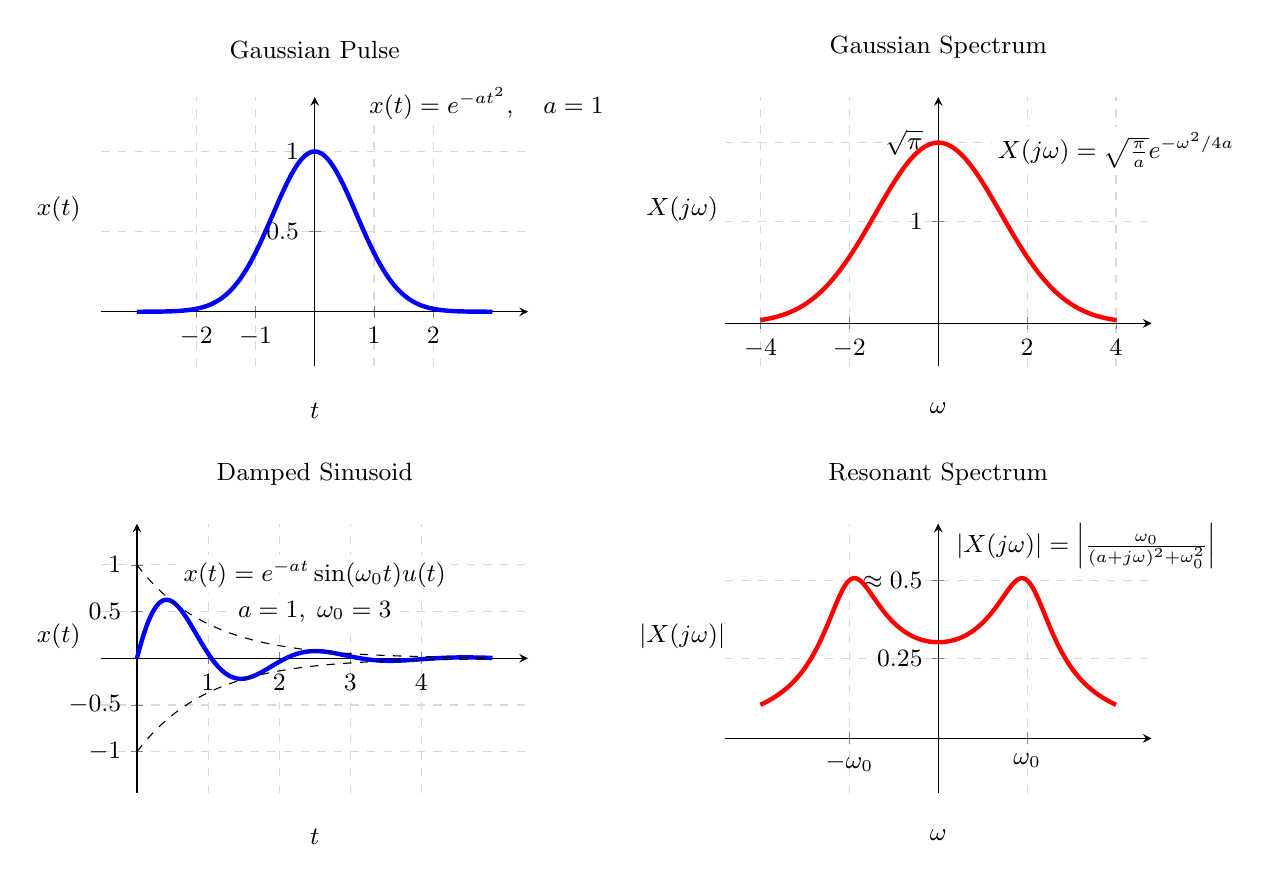
\begin{tikzpicture}
	\begin{groupplot}[
		group style={
			group size=2 by 2,
			horizontal sep=2.5cm,
			vertical sep=2cm
		},
		% Common axis style
		width=7cm,
		height=5cm,
		axis lines=middle,
		enlargelimits=true,
		clip=false,
		xlabel style={at={(axis description cs:0.5,-0.1)},anchor=north},
		ylabel style={at={(axis description cs:-0.1,.5)},anchor=south},
		grid=major,
		grid style={dashed, gray!30},
		samples=300,
		ticklabel style={font=\small},
		every axis/.append style={
			font=\small,
			title style={yshift=1ex},
		}
		]
		
		% PLOT 1: Gaussian pulse (time domain)
		\nextgroupplot[
		title={Gaussian Pulse},
		xlabel={$t$},
		ylabel={$x(t)$},
		xtick={-2,-1,0,1,2},
		ytick={0, 0.5, 1},
		ymin=-0.2,
		ymax=1.2,
		domain=-3:3,
		]
		\addplot[blue, ultra thick] {exp(-x^2)};
		\node[fill=white, inner sep=2pt, font=\small] at (axis cs:2.9,1.3) {$x(t) = e^{-at^2}, \quad a=1$};
		
		% PLOT 2: Gaussian pulse (frequency domain)
		\nextgroupplot[
		title={Gaussian Spectrum},
		xlabel={$\omega$},
		ylabel={$X(j\omega)$},
		domain=-4:4,
		ytick={0, 1, 1.772},
		yticklabels={$0$,$1$,$\sqrt{\pi}$},
		ymin=-0.2,
		ymax=2.0,
		]
		% The FT of exp(-t^2) is sqrt(pi)*exp(-w^2/4)
		\addplot[red, ultra thick] {sqrt(pi)*exp(-x^2/4)};
		\node[fill=white, inner sep=2pt, font=\small] at (axis cs:4, 1.7) {$X(j\omega) = \sqrt{\frac{\pi}{a}} e^{-\omega^2/4a}$};
		
		% PLOT 3: Decaying sinusoid (time domain)
% PLOT 3: Decaying sinusoid (time domain)
\nextgroupplot[
title={Damped Sinusoid},
xlabel={$t$},
ylabel={$x(t)$},
domain=0:5,
xtick={0, 1, 2, 3, 4},
ytick={-1, -0.5, 0, 0.5, 1},
ymin=-1.2,
ymax=1.2,
]
% Plot the signal - radians converted to degrees inside sin
\addplot[blue, ultra thick] {exp(-x)*sin(deg(3*x))};
% Add the decaying envelopes
\addplot[black, dashed, domain=0:5] {exp(-x)};
\addplot[black, dashed, domain=0:5] {-exp(-x)};
\node[fill=white, inner sep=2pt, font=\small] at (axis cs:2.5, 0.9) {$x(t)=e^{-at}\sin(\omega_0 t)u(t)$};
\node[fill=white, inner sep=2pt, font=\small] at (axis cs:2.5, 0.5) {$a=1, \; \omega_0=3$};

		
		% PLOT 4: Decaying sinusoid (frequency domain)
		\nextgroupplot[
		title={Resonant Spectrum},
		xlabel={$\omega$},
		ylabel={$|X(j\omega)|$},
		domain=-6:6,
		xtick={-3, 0, 3},
		xticklabels={$-\omega_0$, $0$, $\omega_0$},
		ytick={0, 0.25, 0.493},
		yticklabels={0, 0.25, $\approx 0.5$},
		ymin=-0.1,
		ymax=0.6,
		]
		% The exact magnitude of the FT for x(t) = e^(-at)sin(w0*t)u(t)
		\addplot[red, ultra thick] {3/sqrt( ( (1^2 - x^2 + 3^2)^2 ) + ( 4*1^2*x^2 ))};
		\node[fill=white, inner sep=2pt, font=\small] at (axis cs:5, 0.6) {$|X(j\omega)| = \left|\frac{\omega_0}{(a+j\omega)^2+\omega_0^2}\right|$};
		
	\end{groupplot}
\end{tikzpicture}
		\caption{Additional CTFT examples: (a) Gaussian pulse, (b) Exponentially decaying sinusoid}
		\label{fig:additional_examples}
	\end{figure}
	\newpage
	\section*{11.4 The Fourier Transform of Periodic Signals}
	
	For periodic signals, the Fourier transform consists of impulses at harmonic frequencies.
	
	\subsection*{11.4.1 Complex Exponential}
	
	You can find the Fourier transform of a complex exponential signal, $x(t) = e^{j\omega_0 t}$, using the same method as for a constant signal: by working backward from the inverse Fourier transform integral. This approach relies on proposing a solution and then proving it works.
	
	
	Let's start by guessing that the Fourier transform, $X(j\omega)$, is a shifted Dirac delta function. The original signal is a "pure" complex sinusoid oscillating at a single frequency, $\omega_0$. Therefore, it's logical to assume that all of its frequency content is concentrated entirely at $\omega = \omega_0$.
	
	Our proposed transform is $X(j\omega) = c \cdot \delta(\omega - \omega_0)$, where $c$ is a constant we need to find.
	
	
	Now, by substituting $X(j\omega) = c \cdot \delta(\omega - \omega_0)$ into the IFT equation:
	\[
	x(t) = \frac{1}{2\pi} \int_{-\infty}^{\infty} [c \cdot \delta(\omega - \omega_0)] e^{j\omega t} \dd\omega
	\]
	 Applying the sifting property, we get:
	\[
	x(t) = \frac{c}{2\pi} e^{j\omega_0 t}
	\]
	
	We want our result to be equal to our original signal, $x(t) = e^{j\omega_0 t}$. By comparing the two, we can see that:
	\[
	\frac{c}{2\pi} = 1 \implies c = 2\pi
	\]
	
 Therefore,
	\[
	e^{j\omega_0 t} \stackrel{\mathcal{F}}{\longleftrightarrow} 2\pi\delta(\omega - \omega_0)
	\]
	
	\subsection*{11.4.2 Sinusoidal Signals}
	
	For $x(t) = \sin(\omega_0 t)$:
	\[
	\sin(\omega_0 t) \stackrel{\mathcal{F}}{\longleftrightarrow} j\pi[\delta(\omega + \omega_0) - \delta(\omega - \omega_0)]
	\]
	
	For $x(t) = \cos(\omega_0 t)$:
	\[
	\cos(\omega_0 t) \stackrel{\mathcal{F}}{\longleftrightarrow} \pi[\delta(\omega + \omega_0) + \delta(\omega - \omega_0)]
	\]
	
	\newpage
	\section*{11.5 Spectrum and Frequency Content}
	
	
	The Fourier transform $X(j\omega)$ represents the \textbf{spectrum} of the signal $x(t)$, showing how the signal's energy is distributed across different frequencies.
	
	\begin{itemize}[noitemsep]
		\item \textbf{Magnitude spectrum} $|X(j\omega)|$: Shows the strength of each frequency component
		\item \textbf{Phase spectrum} $\angle X(j\omega)$: Shows the phase relationship of each frequency component
	\end{itemize}
	
	\section*{11.6 Parseval's Theorem and Energy Conservation}
	
	\begin{theorem}[Parseval's Theorem]
		For a signal $x(t)$ with Fourier transform $X(j\omega)$:
		\[
		\int_{-\infty}^{\infty} |x(t)|^2 \dt = \frac{1}{2\pi} \int_{-\infty}^{\infty} |X(j\omega)|^2 \dd\omega
		\]
	\end{theorem}
	
	This result states that the total energy in a signal is the same whether calculated in the time domain or frequency domain. The quantity $|X(j\omega)|^2$ is called the \textbf{energy spectral density}.
	
	
	
	
	
	\section*{11.7 Examples}
	
	\subsection*{11.7.1 Solved Example}
	
	\begin{example}
		Find the Fourier transform of $x(t) = te^{-a|t|}$ for $a > 0$.
		
		\textbf{Hint:} Write $x(t) = te^{-at}u(t) + te^{at}u(-t)$.
		\[
		X(j\omega) = \frac{1}{(a+j\omega)^2} - \frac{1}{(a-j\omega)^2} = \frac{-4aj\omega}{(a^2 + \omega^2)^2}
		\]
		This result is purely imaginary and odd in $\omega$, because $x(t)$ is real and odd.
	\end{example}
	
	\subsection*{11.7.2 Practice Exercises}
	
	\begin{enumerate}[noitemsep]
		\item Find the CTFT of $x(t) = e^{-|t|}$.
		\item Find the CTFT of $x(t) = \text{rect}(t/T)$ where $\text{rect}(t) = 1$ for $|t| < 1/2$ and $0$ otherwise.
		\item Using Parseval's theorem, find the energy of $x(t) = e^{-at}u(t)$.
		\item Find the CTFT of $x(t) = t^2e^{-at}u(t)$.
		\item Show that if $x(t)$ is real, then $X(-j\omega) = X^*(j\omega)$.
	\end{enumerate}
	
\section*{11.8 Summary and Next Lecture}
	
	The Continuous-Time Fourier Transform extends our frequency-domain analysis to aperiodic signals:
	
	\textbf{Key Takeaways:}
	\begin{itemize}[noitemsep]
		\item \textbf{The CTFT emerges naturally from the CTFS as the period approaches infinity}
		\item \textbf{The analysis equation $X(j\omega) = \int_{-\infty}^{\infty} x(t)e^{-j\omega t} \dt$ extracts frequency content}
		\item \textbf{The synthesis equation $x(t) = \frac{1}{2\pi} \int_{-\infty}^{\infty} X(j\omega)e^{j\omega t} \dd\omega$ reconstructs the signal}
		\item \textbf{The spectrum $X(j\omega)$ provides complete frequency-domain characterization}
		\item \textbf{Convergence is guaranteed by the Dirichlet conditions for most practical signals}
		\item \textbf{Next time:} Properties of the Fourier Transform (linearity, shifting, scaling, duality, convolution)
	\end{itemize}
	
\end{document}
